\section{Durchführung}
\label{sec:Durchführung}

Der Versuch wird gemäß Abbildung \ref{fig:aufbau} aufgebaut. Als Probe wird ein mit Strontium dotierter Kaliumbromid(KBr)-Kristall verwendet.

\begin{figure}
    \centering
    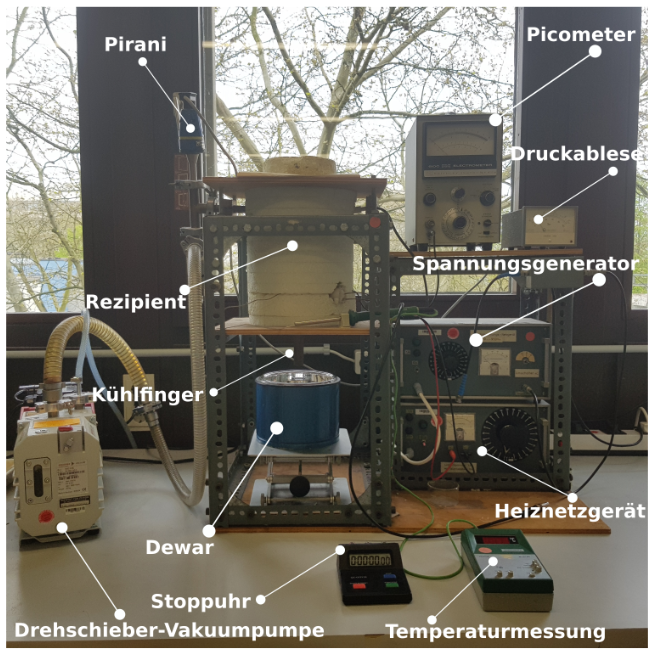
\includegraphics[width=\textwidth]{Bilder/Aufbau.PNG}
    \caption{Aufbau des Versuches.\cite{V48}}
    \label{fig:aufbau}
\end{figure}

Die Probe befindet sich innerhalb eines Plattenkondensators auf der unteren Kondensatorplatte. Der Kondensator ist innerhalb eines Rezipienten (Abbildung \ref{fig:skizze}) mit einem Vakuum von etwa $\SI{0.001}{\milli\bar}$, welches von einer angeschlossenen Vakuumpumpe aufrechtgehalten wird. Ohne das Vakuum würde sich, auf Grund seiner hygroskopischen Eigenschaften, auf dem Kristall eine Wasserschicht bilden. Die Wassermoleküle bilden Dipole, welche sich ihrerseits ebenfalls in dem angelegten E-Feld des Kondensators ausrichten und mit den Dipolen im Kristall wechselwirken. Außerdem beschädigt das Wasser die Kristalloberfläche. Beide Effekte sorgen für Störungen und Ungenauigkeiten in den Messungen.
Um die Temperatur des Kristalls zu beeinflussen, befinden sich am Boden des Rezipienten eine Heizspule und ein Kühlfinger. Die jeweilige Heizrate kann über den Heizstrom reguliert werden. Zum Kühlen wird der Kühlfinger in flüssigen Stickstoff getaucht. Zum Ablesen der aktuellen Temperatur befindet sich ein Thermoelement auf dem Boden des Rezipienten. 


\begin{figure}
    \centering
    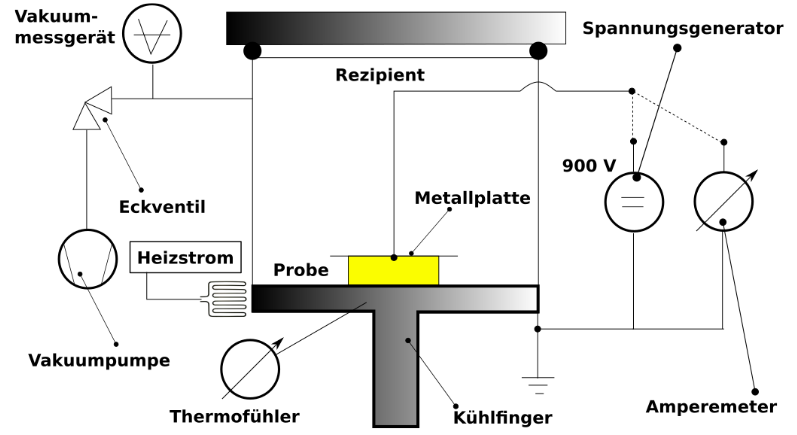
\includegraphics[width=\textwidth]{Bilder/Zeichnung.PNG}
    \caption{Skizzenhafte Darstellung des Aufbaus und Schaltbild der wichtigsten Komponenten.\cite{V48}}
    \label{fig:skizze}
\end{figure}


Als erstes wird ein E-Feld im Kondensator mit einer Spannung von $\SI{950}{\volt}$ erzeugt. Zeitgleich wird der Kristall auf ca $\SI{55}{\celsius}$ erhitzt. Nach einer außreichend langen Zeit (ca. $\SI{900}{\second}$) wird der Kühlfinger in flüssigen Stickstoff getaucht, um so den Kristall auf $\SI{-80}{\celsius}$ abzukühlen. Sobald die Temperatur erreicht ist, wird das E-Feld abgestellt und der Kondensator für $\SI{6}{\minute}$ kurzgeschlossen. Daraufhin beginnen die Messungen.


Bei einer möglichst konstant gehaltenen Heizrate von $\SI{1.5}{\celsius\per\minute}$ wird pro Minute die herrschende Temperatur und der aktuelle Strom notiert. Diese/r lässt sich vom Thermoelement bzw. vom Amperemeter ablesen. Dabei ist der Stom gemeint, welcher durch die Dipolrelaxation innerhalb des Kristalls erzeugt wird und durch die in Abbildung \ref{fig:skizze} dargestellte Schaltung fließt. Während der Messungen gilt es möglichst wenige große oder schnelle Bewegungen durchzuführen. Diese würden bereits die feinen Messungen des Stroms stören, da sie ihrerseits einen zusätzlichen Strom induzieren würden. 
Der ganze Prozess des Erhitzens, E-Feld erzeugen, Abkühlen etc. wird mit einer Heizrate von diesmal $\SI{2}{\celsius\per\minute}$ wiederholt.

%Was wurde gemessen bzw. welche Größen wurden variiert?